\documentclass[11pt]{article}
\usepackage[textwidth=18.0cm, textheight=23.0cm, top=2.0cm]{geometry}
\usepackage{pst-all}
\usepackage{amssymb}
\usepackage{tikz}
\usepackage{underscore}\begin{document}
\pagestyle{empty}


ClassName: \underline{\textbf{Class_08.2bp-24}}
\par
BinSize: \underline{\textbf{100 × 100}}
\par
ReduceSize: \underline{\textbf{100 × 100}}
\par
TypeNum: \underline{\textbf{59}}
\par
Num: \underline{\textbf{60}}
\par
OutS: \underline{\textbf{140000}}
\par
InS: \underline{\textbf{121885}}
\par
Rate: \underline{\textbf{0.871}}
\par
UB: \underline{\textbf{14}}
\par
LB0: \underline{\textbf{14}}
\par
LB: \underline{\textbf{14}}
\par
LBWithCut: \underline{\textbf{14}}
\par
NodeCut: \underline{\textbf{0}}
\par
ExtendedNodeCnt: \underline{\textbf{1}}
\par
GenNodeCnt: \underline{\textbf{1}}
\par
PrimalNode: \underline{\textbf{0}}
\par
ColumnCount: \underline{\textbf{14}}
\par
TotalCutCount: \underline{\textbf{0}}
\par
RootCutCount: \underline{\textbf{0}}
\par
LPSolverCnt: \underline{\textbf{1}}
\par
PricingSolverCnt: \underline{\textbf{0}}
\par
BranchAndBoundNum: \underline{\textbf{1}}
\par
isOpt: \underline{\textbf{true}}
\par
TimeOnInitSolution: \underline{\textbf{600.000 s}}
\par
TimeOnPrimal: \underline{\textbf{0.000 s}}
\par
TimeOnPricing: \underline{\textbf{0.000 s}}
\par
TimeOnRmp: \underline{\textbf{0.094 s}}
\par
TotalTime: \underline{\textbf{600.360 s}}
\par
\newpage


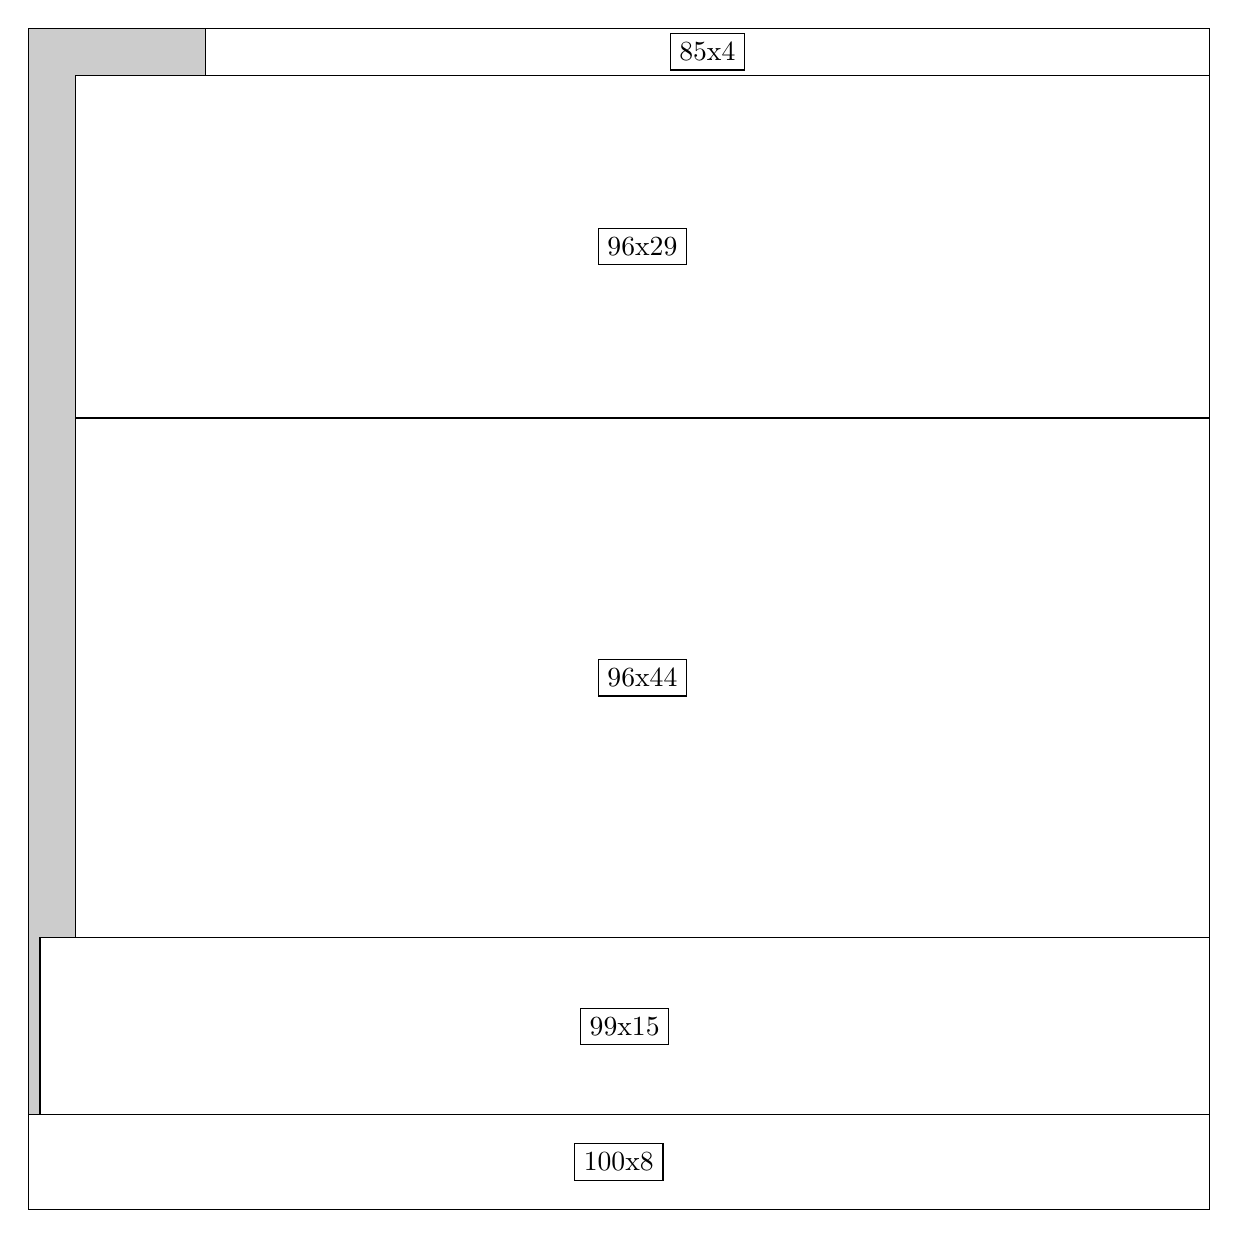
\begin{tikzpicture}[shorten >=1pt,scale=1.0,every node/.style={scale=1.0},->]
\tikzstyle{vertex}=[circle,fill=black!25,minimum size=14pt,inner sep=0pt]
\filldraw[fill=gray!40!white, draw=black] (0,0) rectangle (15.0,15.0);
\foreach \name/\x/\y/\w/\h in {100x8/0.0/0.0/15.0/1.2,99x15/0.15/1.2/14.85/2.25,96x44/0.6/3.4499999999999997/14.399999999999999/6.6,96x29/0.6/10.049999999999999/14.399999999999999/4.35,85x4/2.25/14.399999999999999/12.75/0.6}
\filldraw[fill=white!40!white, draw=black] (\x,\y) rectangle node[draw] (\name) {\name} ++(\w,\h);
\end{tikzpicture}


w =100 , h =8 , x =0 , y =0 , v =800
\par
w =99 , h =15 , x =1 , y =8 , v =1485
\par
w =96 , h =44 , x =4 , y =23 , v =4224
\par
w =96 , h =29 , x =4 , y =67 , v =2784
\par
w =85 , h =4 , x =15 , y =96 , v =340
\par
\newpage


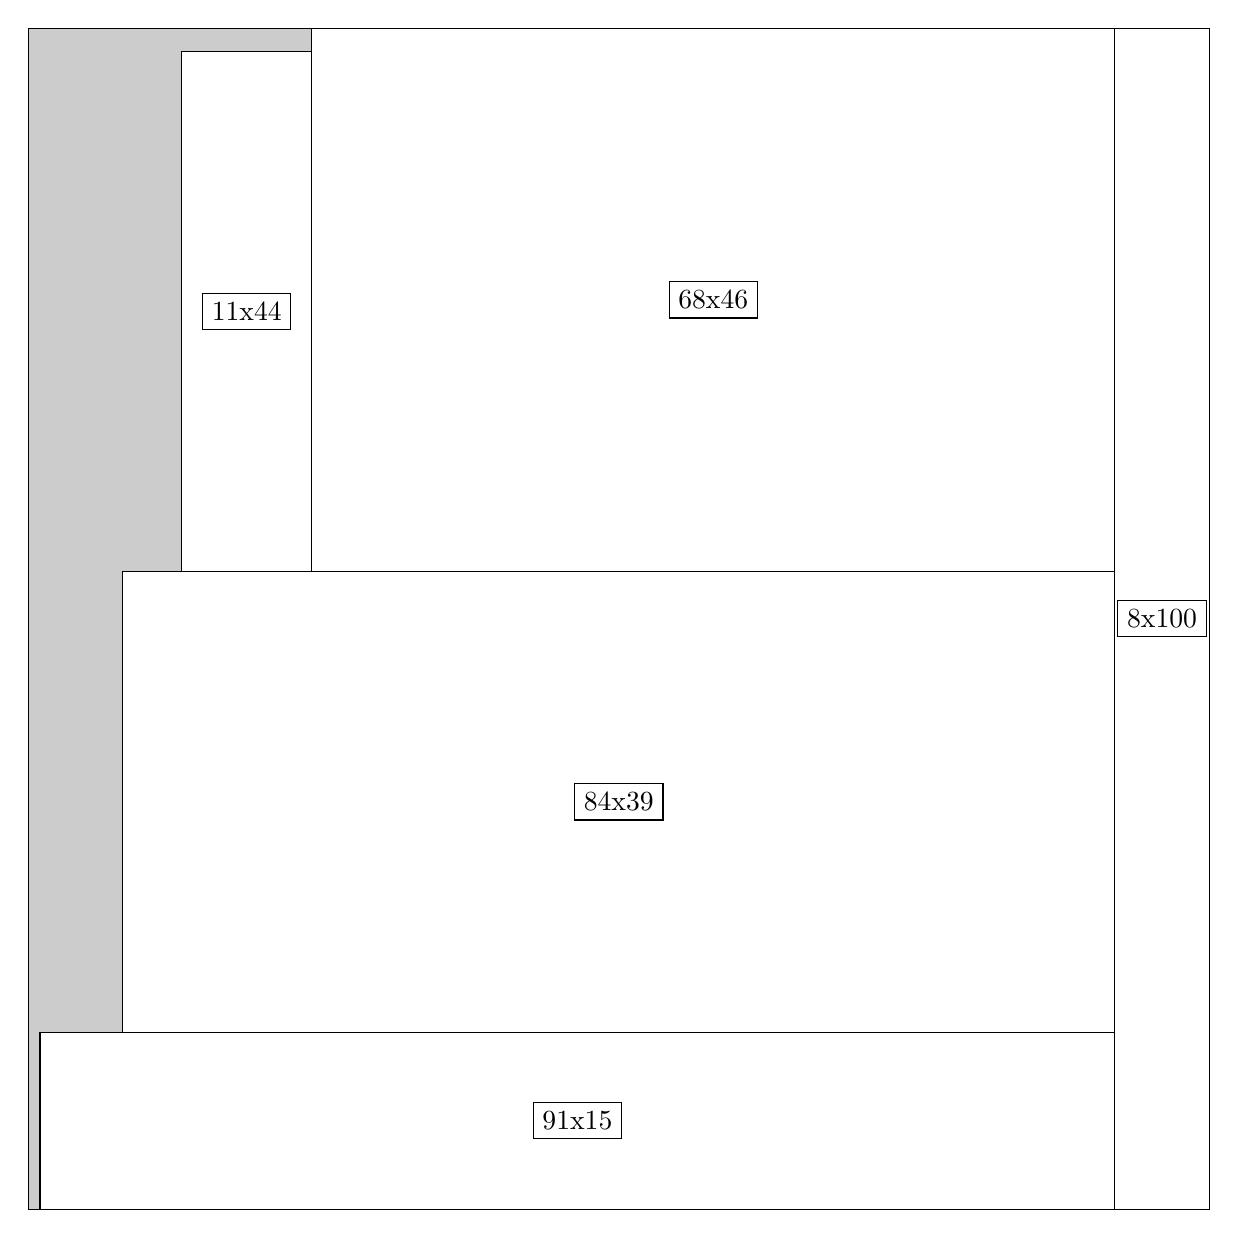
\begin{tikzpicture}[shorten >=1pt,scale=1.0,every node/.style={scale=1.0},->]
\tikzstyle{vertex}=[circle,fill=black!25,minimum size=14pt,inner sep=0pt]
\filldraw[fill=gray!40!white, draw=black] (0,0) rectangle (15.0,15.0);
\foreach \name/\x/\y/\w/\h in {8x100/13.799999999999999/0.0/1.2/15.0,91x15/0.15/0.0/13.65/2.25,84x39/1.2/2.25/12.6/5.85,68x46/3.5999999999999996/8.1/10.2/6.8999999999999995,11x44/1.95/8.1/1.65/6.6}
\filldraw[fill=white!40!white, draw=black] (\x,\y) rectangle node[draw] (\name) {\name} ++(\w,\h);
\end{tikzpicture}


w =8 , h =100 , x =92 , y =0 , v =800
\par
w =91 , h =15 , x =1 , y =0 , v =1365
\par
w =84 , h =39 , x =8 , y =15 , v =3276
\par
w =68 , h =46 , x =24 , y =54 , v =3128
\par
w =11 , h =44 , x =13 , y =54 , v =484
\par
\newpage


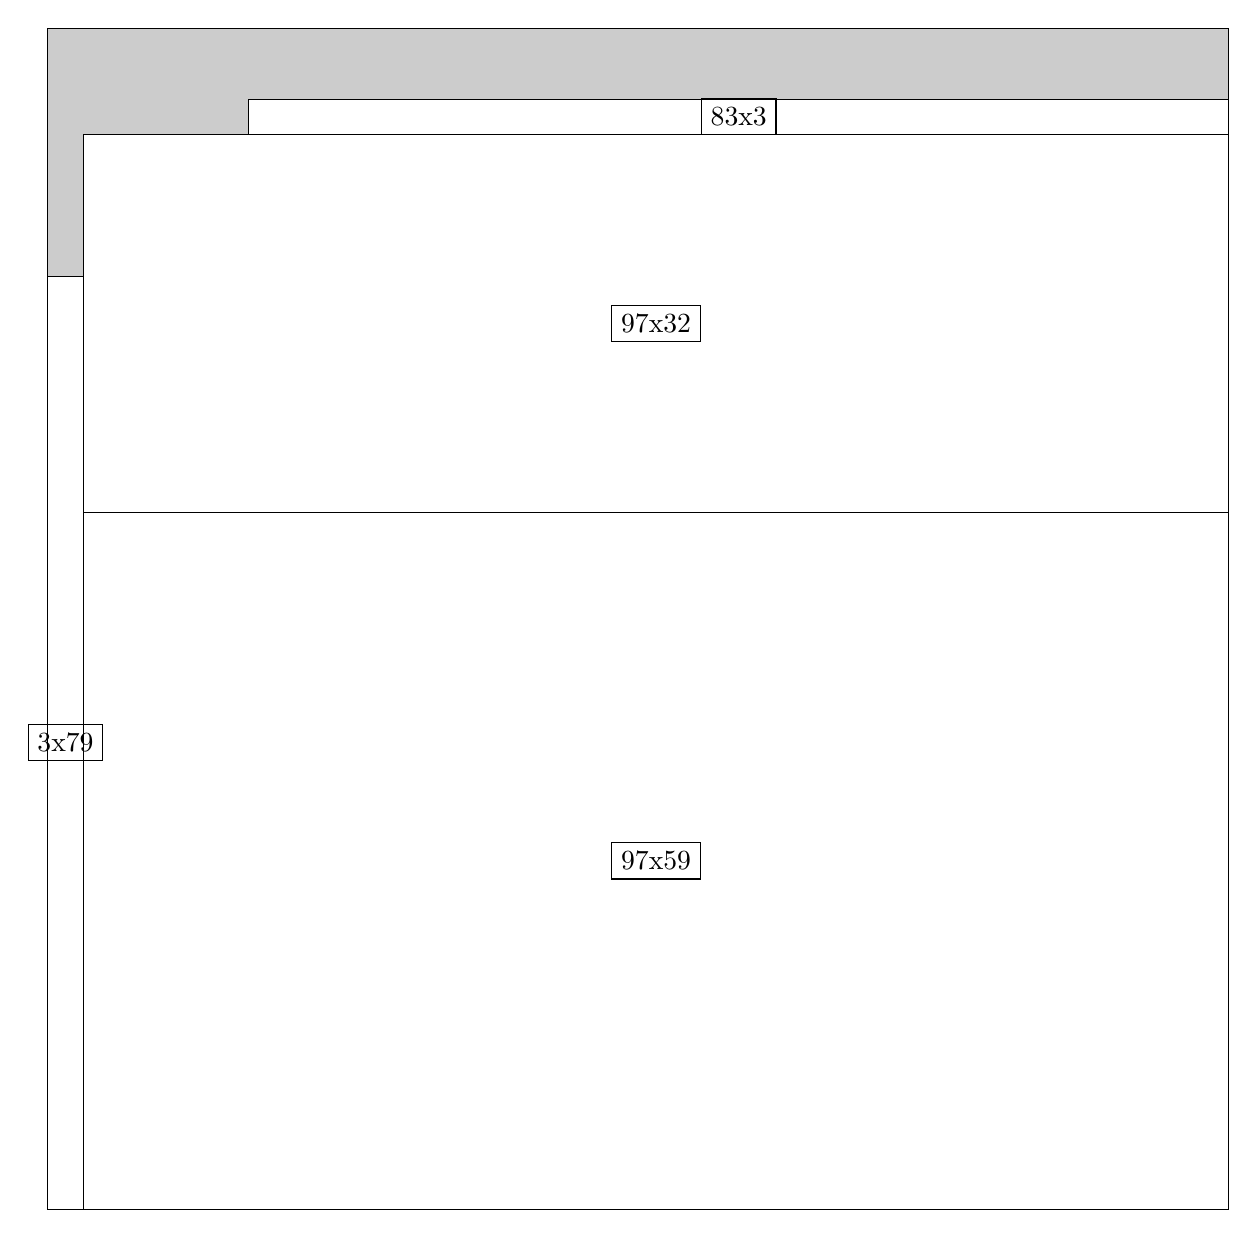
\begin{tikzpicture}[shorten >=1pt,scale=1.0,every node/.style={scale=1.0},->]
\tikzstyle{vertex}=[circle,fill=black!25,minimum size=14pt,inner sep=0pt]
\filldraw[fill=gray!40!white, draw=black] (0,0) rectangle (15.0,15.0);
\foreach \name/\x/\y/\w/\h in {97x59/0.44999999999999996/0.0/14.549999999999999/8.85,97x32/0.44999999999999996/8.85/14.549999999999999/4.8,83x3/2.55/13.65/12.45/0.44999999999999996,3x79/0.0/0.0/0.44999999999999996/11.85}
\filldraw[fill=white!40!white, draw=black] (\x,\y) rectangle node[draw] (\name) {\name} ++(\w,\h);
\end{tikzpicture}


w =97 , h =59 , x =3 , y =0 , v =5723
\par
w =97 , h =32 , x =3 , y =59 , v =3104
\par
w =83 , h =3 , x =17 , y =91 , v =249
\par
w =3 , h =79 , x =0 , y =0 , v =237
\par
\newpage


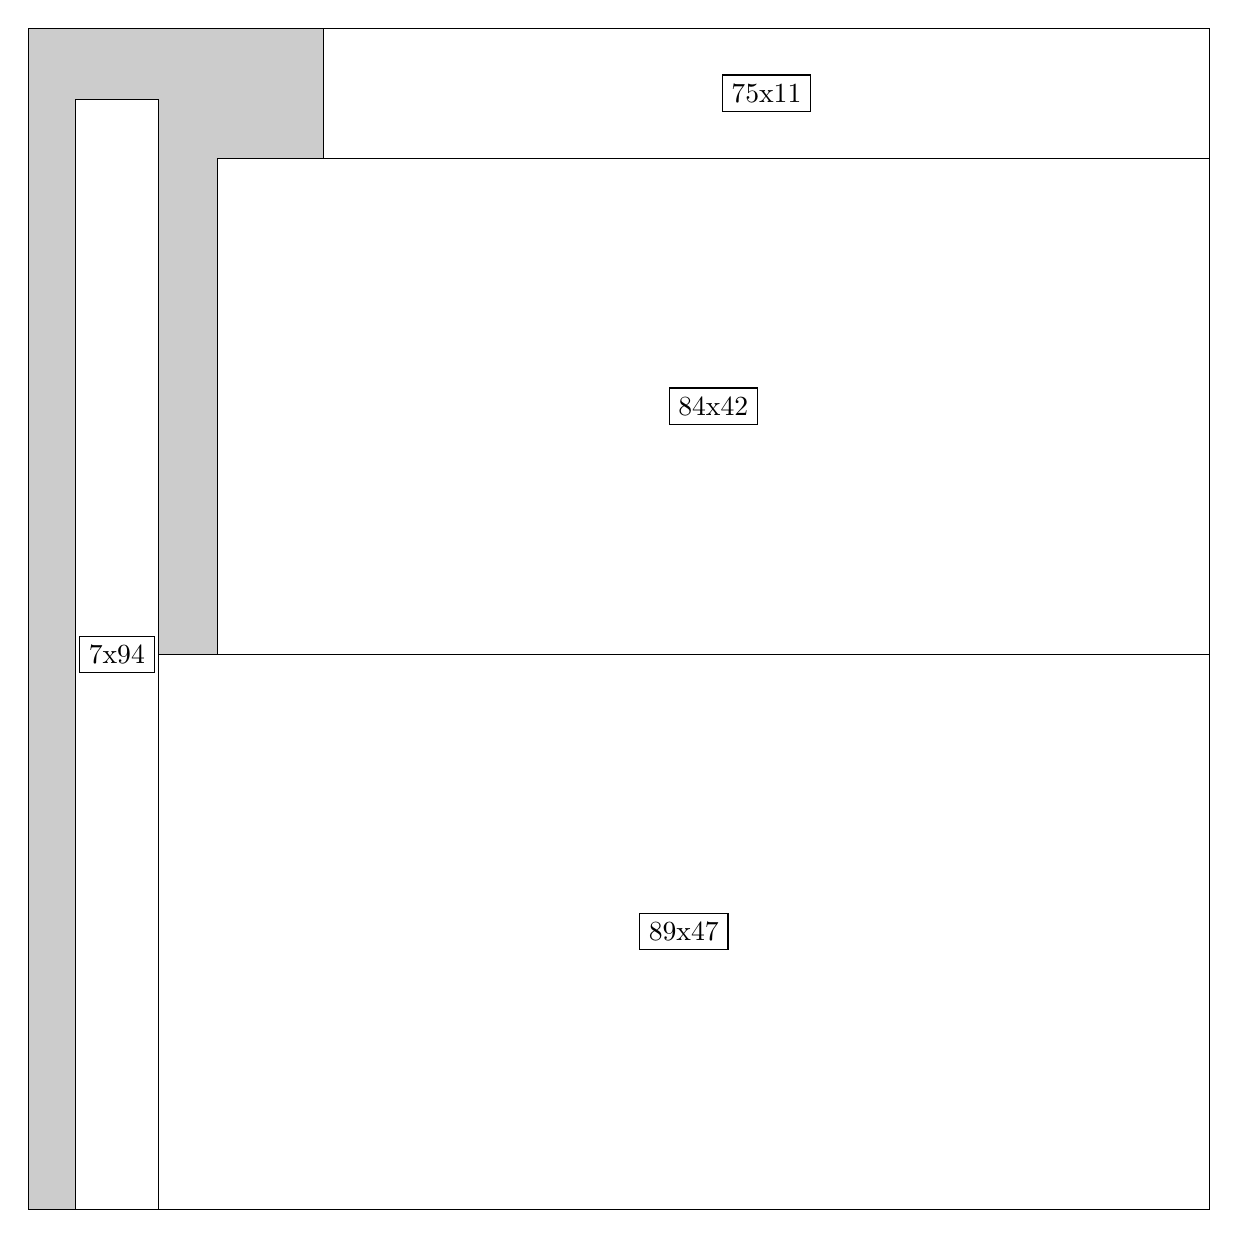
\begin{tikzpicture}[shorten >=1pt,scale=1.0,every node/.style={scale=1.0},->]
\tikzstyle{vertex}=[circle,fill=black!25,minimum size=14pt,inner sep=0pt]
\filldraw[fill=gray!40!white, draw=black] (0,0) rectangle (15.0,15.0);
\foreach \name/\x/\y/\w/\h in {89x47/1.65/0.0/13.35/7.05,84x42/2.4/7.05/12.6/6.3,75x11/3.75/13.35/11.25/1.65,7x94/0.6/0.0/1.05/14.1}
\filldraw[fill=white!40!white, draw=black] (\x,\y) rectangle node[draw] (\name) {\name} ++(\w,\h);
\end{tikzpicture}


w =89 , h =47 , x =11 , y =0 , v =4183
\par
w =84 , h =42 , x =16 , y =47 , v =3528
\par
w =75 , h =11 , x =25 , y =89 , v =825
\par
w =7 , h =94 , x =4 , y =0 , v =658
\par
\newpage


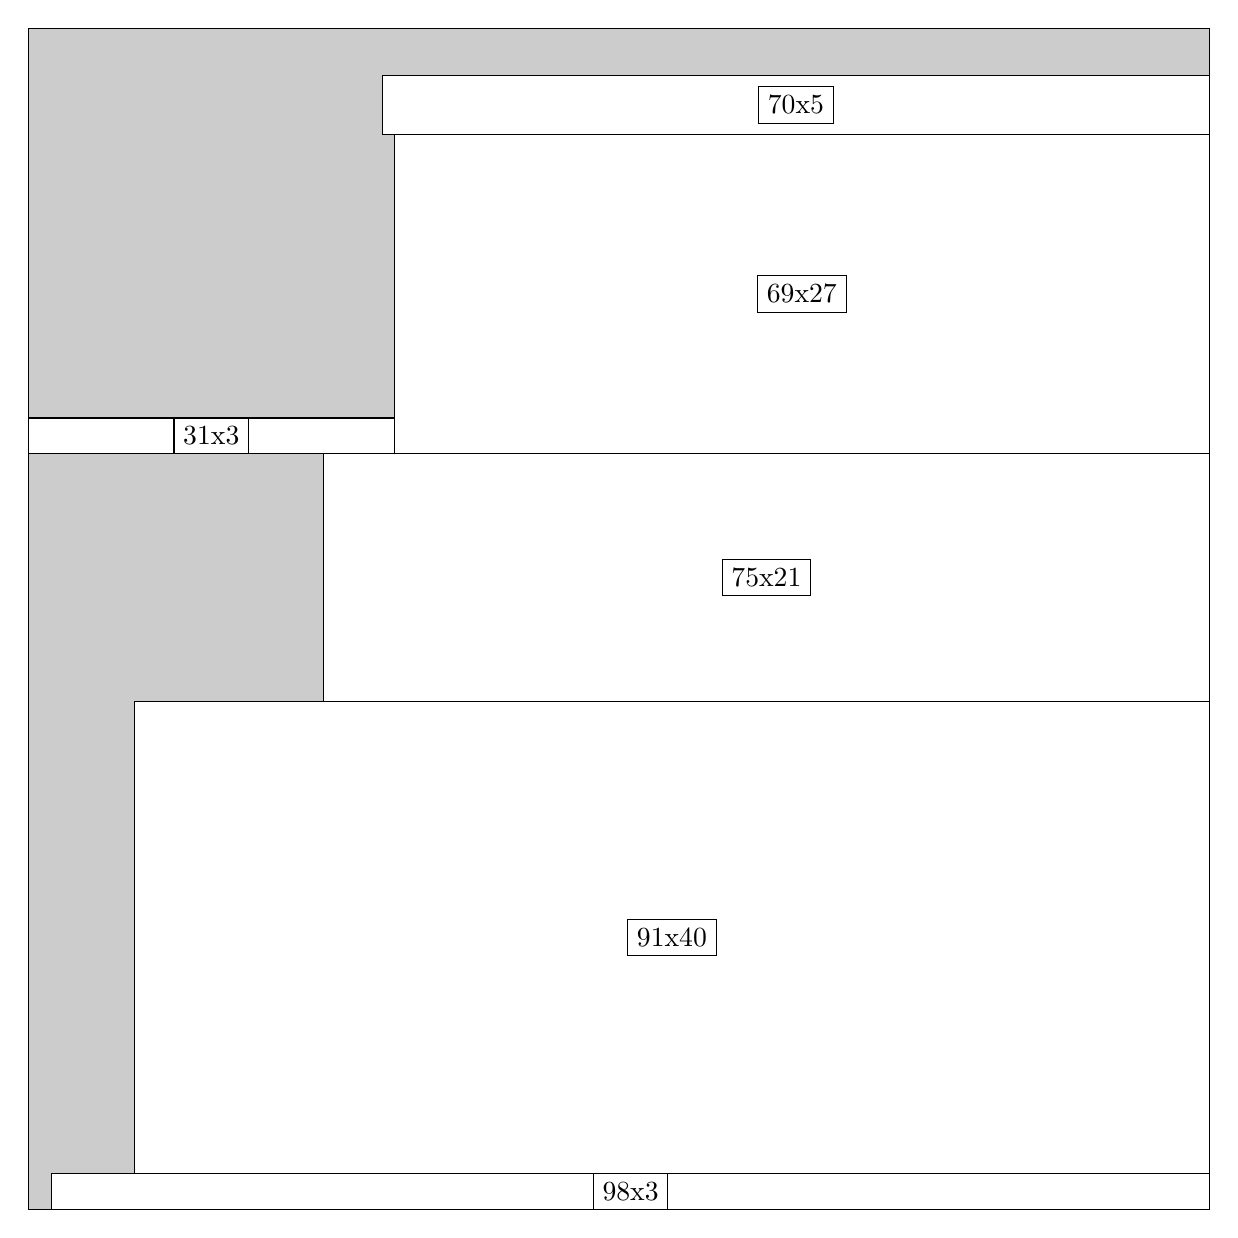
\begin{tikzpicture}[shorten >=1pt,scale=1.0,every node/.style={scale=1.0},->]
\tikzstyle{vertex}=[circle,fill=black!25,minimum size=14pt,inner sep=0pt]
\filldraw[fill=gray!40!white, draw=black] (0,0) rectangle (15.0,15.0);
\foreach \name/\x/\y/\w/\h in {98x3/0.3/0.0/14.7/0.44999999999999996,91x40/1.3499999999999999/0.44999999999999996/13.65/6.0,75x21/3.75/6.45/11.25/3.15,69x27/4.6499999999999995/9.6/10.35/4.05,31x3/0.0/9.6/4.6499999999999995/0.44999999999999996,70x5/4.5/13.65/10.5/0.75}
\filldraw[fill=white!40!white, draw=black] (\x,\y) rectangle node[draw] (\name) {\name} ++(\w,\h);
\end{tikzpicture}


w =98 , h =3 , x =2 , y =0 , v =294
\par
w =91 , h =40 , x =9 , y =3 , v =3640
\par
w =75 , h =21 , x =25 , y =43 , v =1575
\par
w =69 , h =27 , x =31 , y =64 , v =1863
\par
w =31 , h =3 , x =0 , y =64 , v =93
\par
w =70 , h =5 , x =30 , y =91 , v =350
\par
\newpage


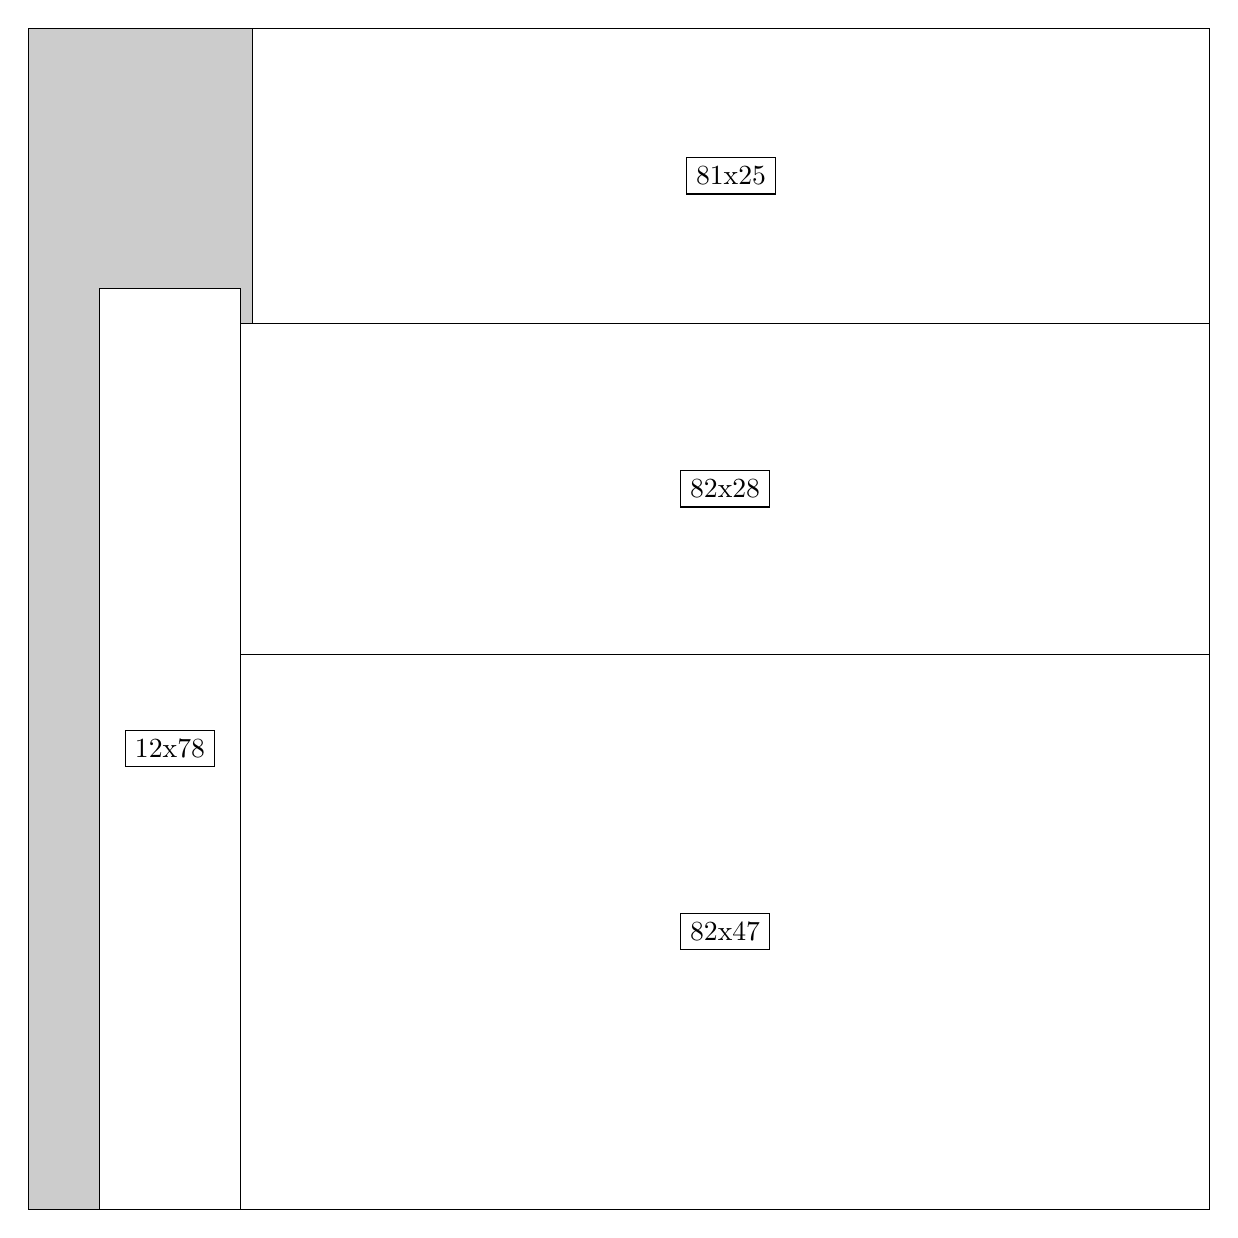
\begin{tikzpicture}[shorten >=1pt,scale=1.0,every node/.style={scale=1.0},->]
\tikzstyle{vertex}=[circle,fill=black!25,minimum size=14pt,inner sep=0pt]
\filldraw[fill=gray!40!white, draw=black] (0,0) rectangle (15.0,15.0);
\foreach \name/\x/\y/\w/\h in {82x47/2.6999999999999997/0.0/12.299999999999999/7.05,82x28/2.6999999999999997/7.05/12.299999999999999/4.2,81x25/2.85/11.25/12.15/3.75,12x78/0.8999999999999999/0.0/1.7999999999999998/11.7}
\filldraw[fill=white!40!white, draw=black] (\x,\y) rectangle node[draw] (\name) {\name} ++(\w,\h);
\end{tikzpicture}


w =82 , h =47 , x =18 , y =0 , v =3854
\par
w =82 , h =28 , x =18 , y =47 , v =2296
\par
w =81 , h =25 , x =19 , y =75 , v =2025
\par
w =12 , h =78 , x =6 , y =0 , v =936
\par
\newpage


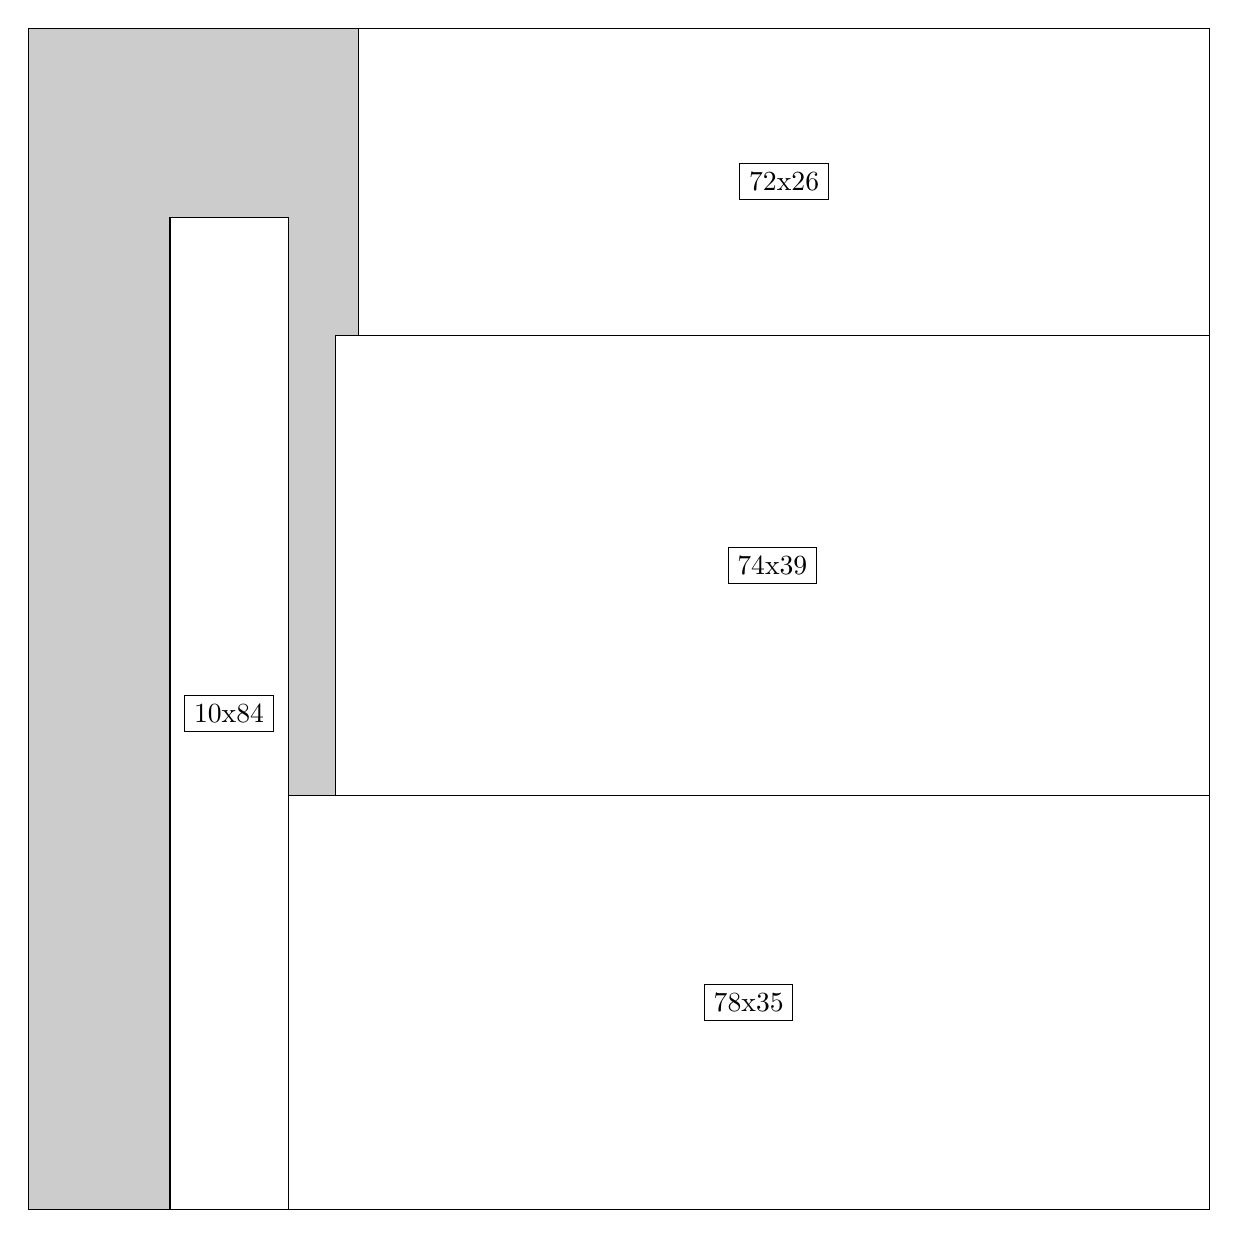
\begin{tikzpicture}[shorten >=1pt,scale=1.0,every node/.style={scale=1.0},->]
\tikzstyle{vertex}=[circle,fill=black!25,minimum size=14pt,inner sep=0pt]
\filldraw[fill=gray!40!white, draw=black] (0,0) rectangle (15.0,15.0);
\foreach \name/\x/\y/\w/\h in {78x35/3.3/0.0/11.7/5.25,74x39/3.9/5.25/11.1/5.85,72x26/4.2/11.1/10.799999999999999/3.9,10x84/1.7999999999999998/0.0/1.5/12.6}
\filldraw[fill=white!40!white, draw=black] (\x,\y) rectangle node[draw] (\name) {\name} ++(\w,\h);
\end{tikzpicture}


w =78 , h =35 , x =22 , y =0 , v =2730
\par
w =74 , h =39 , x =26 , y =35 , v =2886
\par
w =72 , h =26 , x =28 , y =74 , v =1872
\par
w =10 , h =84 , x =12 , y =0 , v =840
\par
\newpage


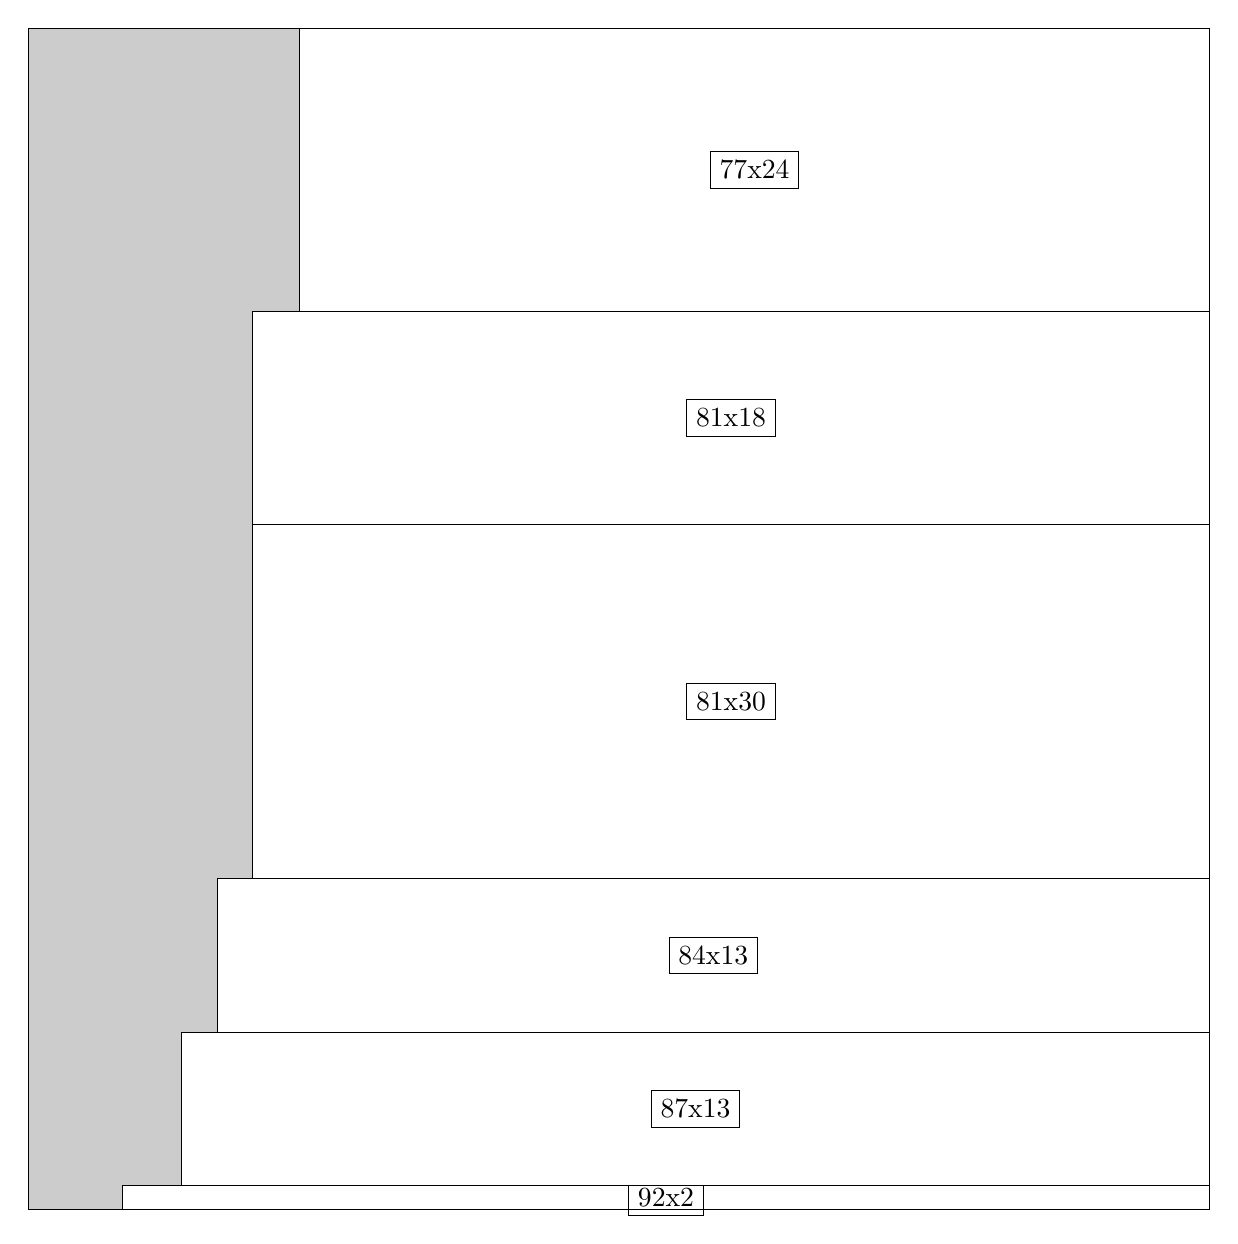
\begin{tikzpicture}[shorten >=1pt,scale=1.0,every node/.style={scale=1.0},->]
\tikzstyle{vertex}=[circle,fill=black!25,minimum size=14pt,inner sep=0pt]
\filldraw[fill=gray!40!white, draw=black] (0,0) rectangle (15.0,15.0);
\foreach \name/\x/\y/\w/\h in {92x2/1.2/0.0/13.799999999999999/0.3,87x13/1.95/0.3/13.049999999999999/1.95,84x13/2.4/2.25/12.6/1.95,81x30/2.85/4.2/12.15/4.5,81x18/2.85/8.7/12.15/2.6999999999999997,77x24/3.4499999999999997/11.4/11.549999999999999/3.5999999999999996}
\filldraw[fill=white!40!white, draw=black] (\x,\y) rectangle node[draw] (\name) {\name} ++(\w,\h);
\end{tikzpicture}


w =92 , h =2 , x =8 , y =0 , v =184
\par
w =87 , h =13 , x =13 , y =2 , v =1131
\par
w =84 , h =13 , x =16 , y =15 , v =1092
\par
w =81 , h =30 , x =19 , y =28 , v =2430
\par
w =81 , h =18 , x =19 , y =58 , v =1458
\par
w =77 , h =24 , x =23 , y =76 , v =1848
\par
\newpage


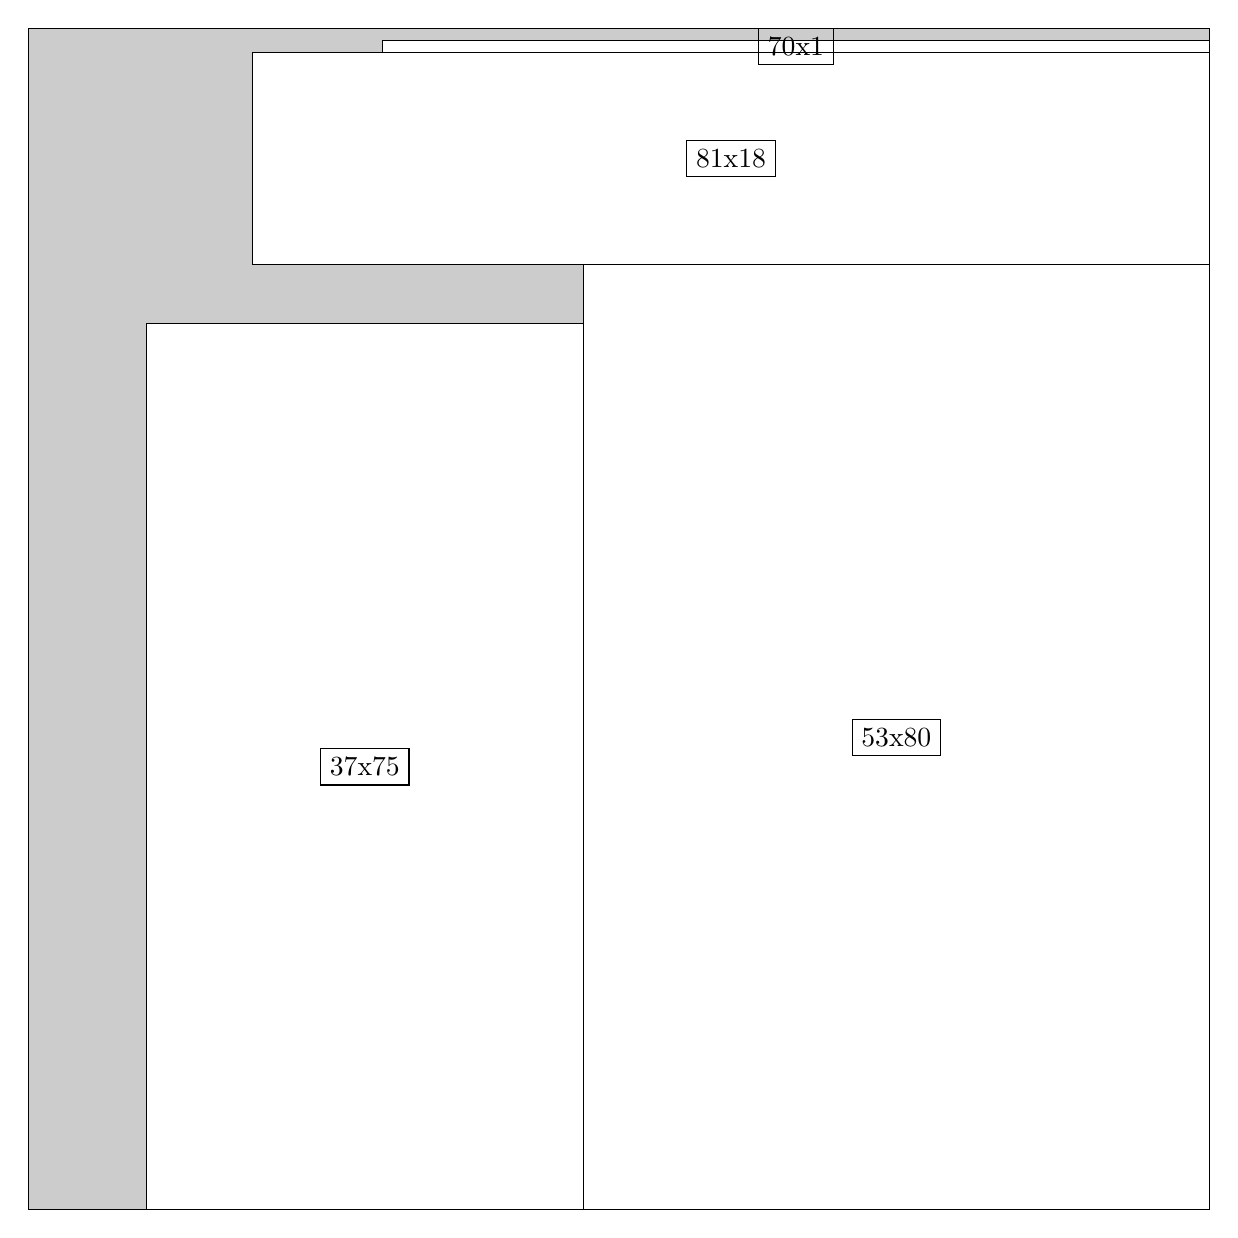
\begin{tikzpicture}[shorten >=1pt,scale=1.0,every node/.style={scale=1.0},->]
\tikzstyle{vertex}=[circle,fill=black!25,minimum size=14pt,inner sep=0pt]
\filldraw[fill=gray!40!white, draw=black] (0,0) rectangle (15.0,15.0);
\foreach \name/\x/\y/\w/\h in {53x80/7.05/0.0/7.949999999999999/12.0,37x75/1.5/0.0/5.55/11.25,81x18/2.85/12.0/12.15/2.6999999999999997,70x1/4.5/14.7/10.5/0.15}
\filldraw[fill=white!40!white, draw=black] (\x,\y) rectangle node[draw] (\name) {\name} ++(\w,\h);
\end{tikzpicture}


w =53 , h =80 , x =47 , y =0 , v =4240
\par
w =37 , h =75 , x =10 , y =0 , v =2775
\par
w =81 , h =18 , x =19 , y =80 , v =1458
\par
w =70 , h =1 , x =30 , y =98 , v =70
\par
\newpage


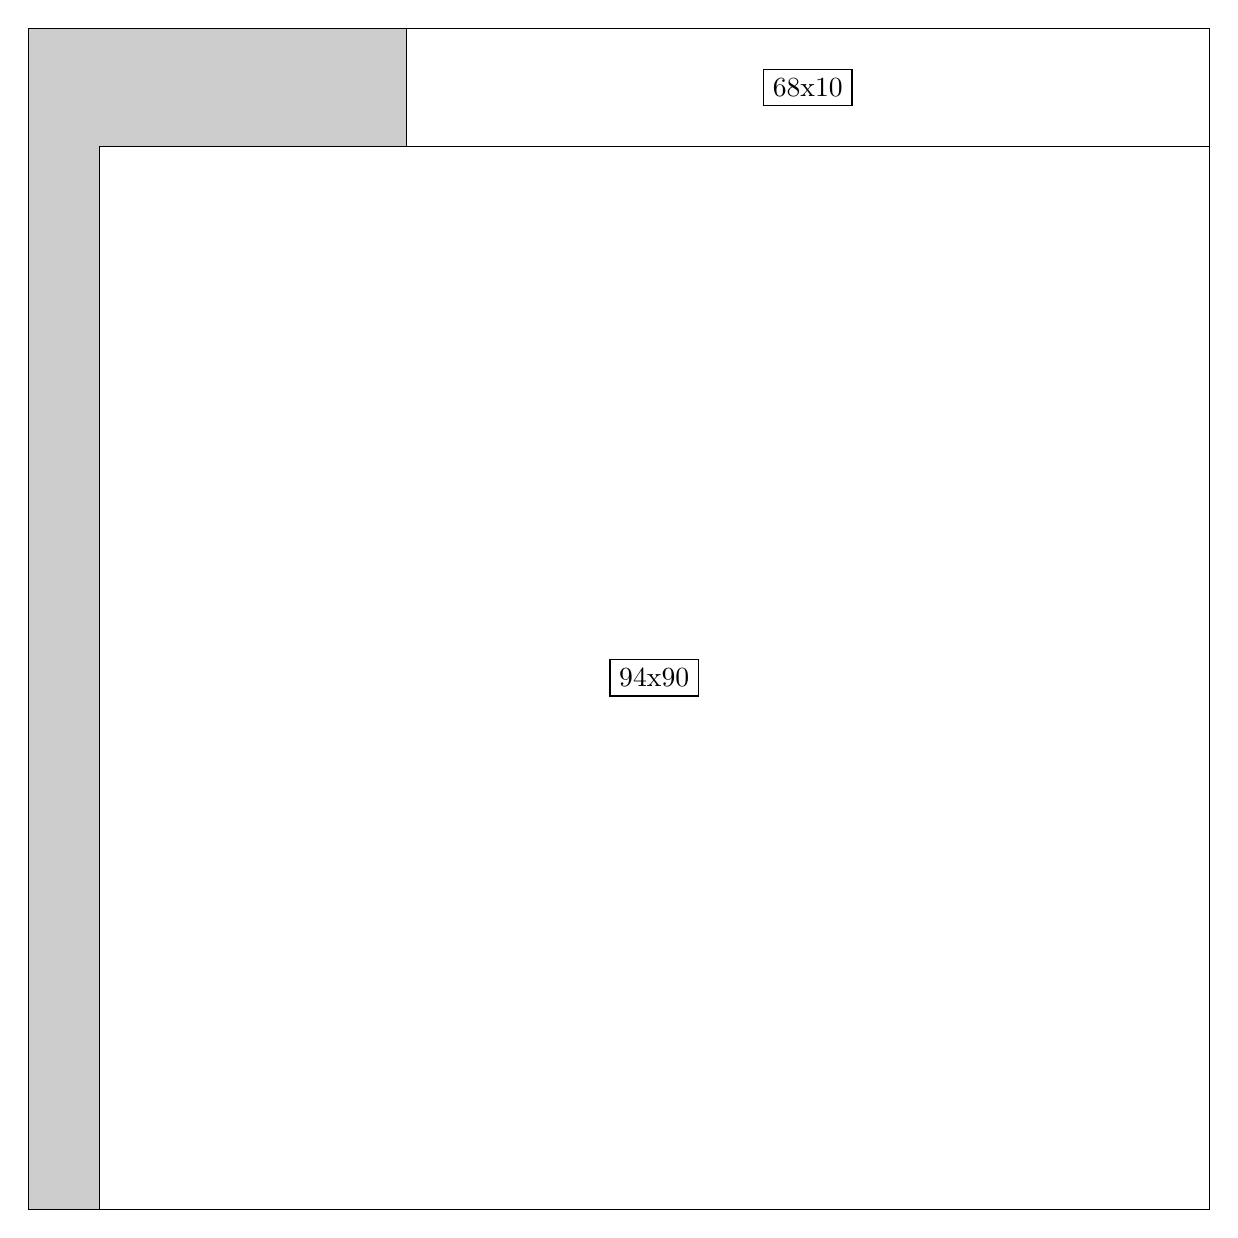
\begin{tikzpicture}[shorten >=1pt,scale=1.0,every node/.style={scale=1.0},->]
\tikzstyle{vertex}=[circle,fill=black!25,minimum size=14pt,inner sep=0pt]
\filldraw[fill=gray!40!white, draw=black] (0,0) rectangle (15.0,15.0);
\foreach \name/\x/\y/\w/\h in {94x90/0.8999999999999999/0.0/14.1/13.5,68x10/4.8/13.5/10.2/1.5}
\filldraw[fill=white!40!white, draw=black] (\x,\y) rectangle node[draw] (\name) {\name} ++(\w,\h);
\end{tikzpicture}


w =94 , h =90 , x =6 , y =0 , v =8460
\par
w =68 , h =10 , x =32 , y =90 , v =680
\par
\newpage


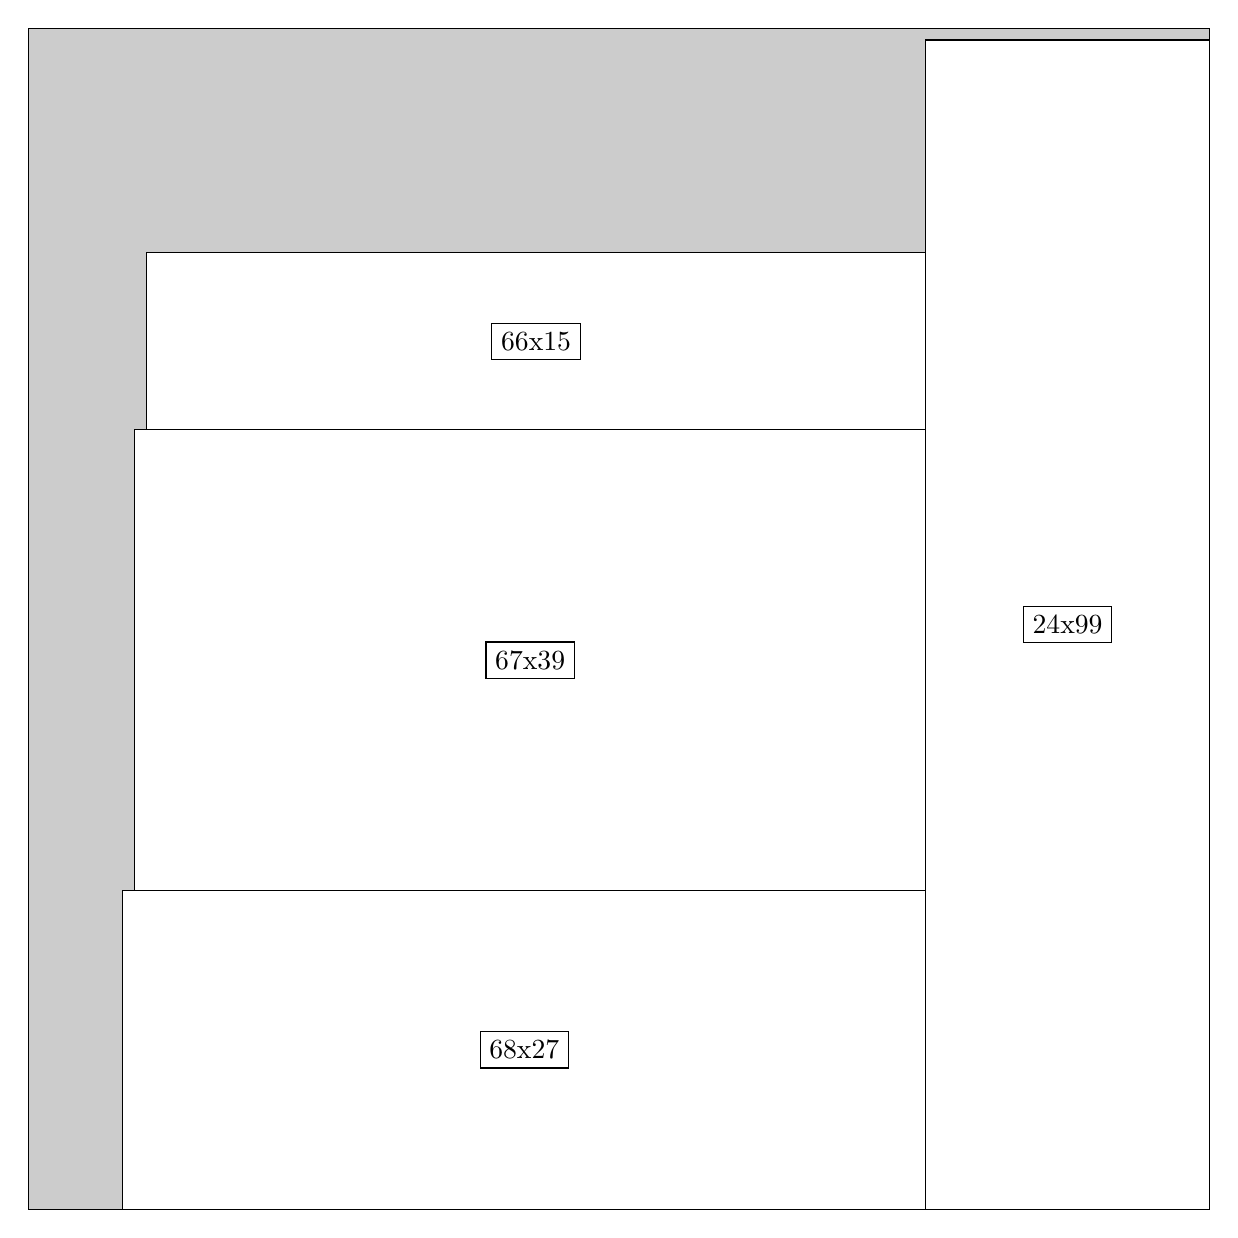
\begin{tikzpicture}[shorten >=1pt,scale=1.0,every node/.style={scale=1.0},->]
\tikzstyle{vertex}=[circle,fill=black!25,minimum size=14pt,inner sep=0pt]
\filldraw[fill=gray!40!white, draw=black] (0,0) rectangle (15.0,15.0);
\foreach \name/\x/\y/\w/\h in {24x99/11.4/0.0/3.5999999999999996/14.85,68x27/1.2/0.0/10.2/4.05,67x39/1.3499999999999999/4.05/10.049999999999999/5.85,66x15/1.5/9.9/9.9/2.25}
\filldraw[fill=white!40!white, draw=black] (\x,\y) rectangle node[draw] (\name) {\name} ++(\w,\h);
\end{tikzpicture}


w =24 , h =99 , x =76 , y =0 , v =2376
\par
w =68 , h =27 , x =8 , y =0 , v =1836
\par
w =67 , h =39 , x =9 , y =27 , v =2613
\par
w =66 , h =15 , x =10 , y =66 , v =990
\par
\newpage


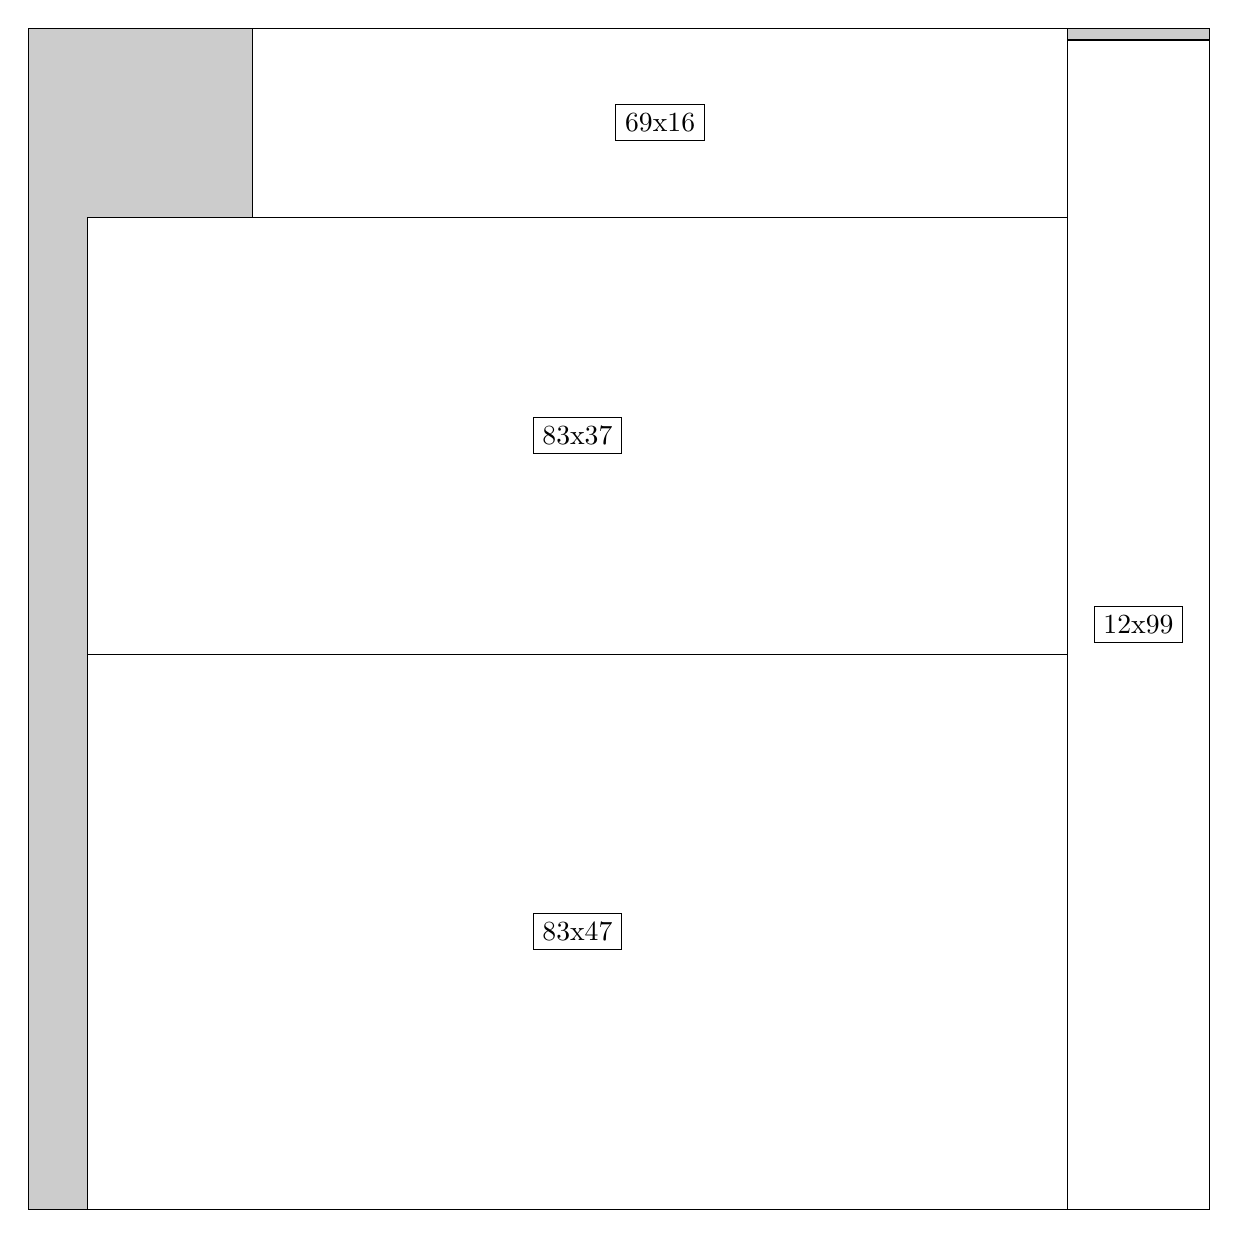
\begin{tikzpicture}[shorten >=1pt,scale=1.0,every node/.style={scale=1.0},->]
\tikzstyle{vertex}=[circle,fill=black!25,minimum size=14pt,inner sep=0pt]
\filldraw[fill=gray!40!white, draw=black] (0,0) rectangle (15.0,15.0);
\foreach \name/\x/\y/\w/\h in {12x99/13.2/0.0/1.7999999999999998/14.85,83x47/0.75/0.0/12.45/7.05,83x37/0.75/7.05/12.45/5.55,69x16/2.85/12.6/10.35/2.4}
\filldraw[fill=white!40!white, draw=black] (\x,\y) rectangle node[draw] (\name) {\name} ++(\w,\h);
\end{tikzpicture}


w =12 , h =99 , x =88 , y =0 , v =1188
\par
w =83 , h =47 , x =5 , y =0 , v =3901
\par
w =83 , h =37 , x =5 , y =47 , v =3071
\par
w =69 , h =16 , x =19 , y =84 , v =1104
\par
\newpage


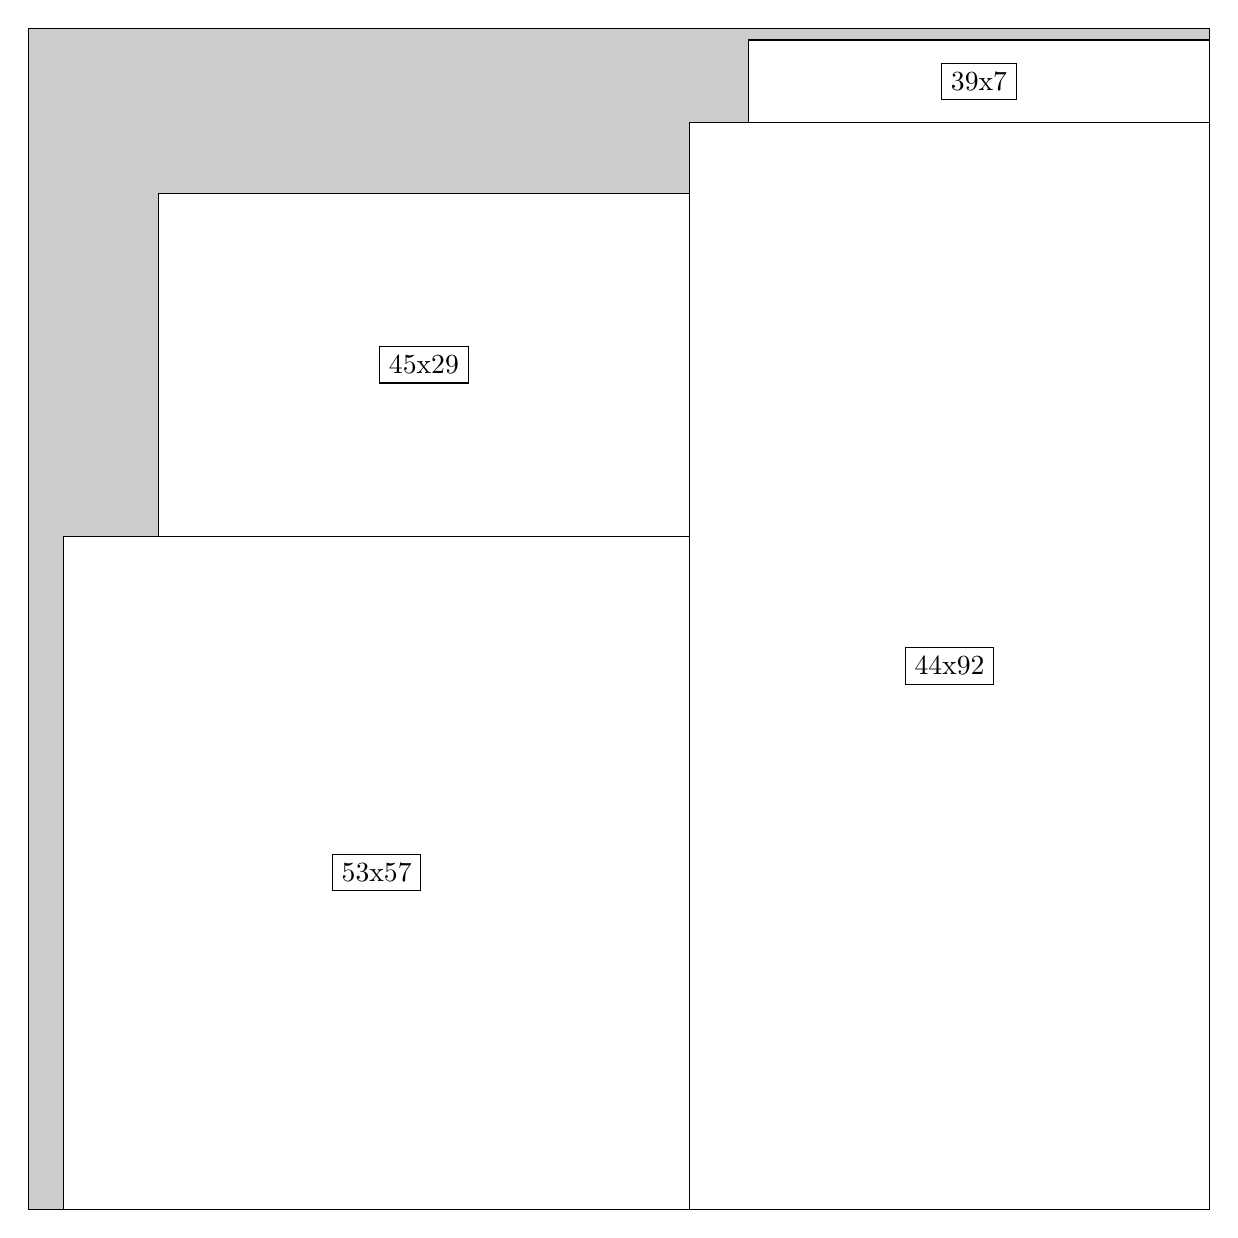
\begin{tikzpicture}[shorten >=1pt,scale=1.0,every node/.style={scale=1.0},->]
\tikzstyle{vertex}=[circle,fill=black!25,minimum size=14pt,inner sep=0pt]
\filldraw[fill=gray!40!white, draw=black] (0,0) rectangle (15.0,15.0);
\foreach \name/\x/\y/\w/\h in {44x92/8.4/0.0/6.6/13.799999999999999,53x57/0.44999999999999996/0.0/7.949999999999999/8.549999999999999,45x29/1.65/8.549999999999999/6.75/4.35,39x7/9.15/13.799999999999999/5.85/1.05}
\filldraw[fill=white!40!white, draw=black] (\x,\y) rectangle node[draw] (\name) {\name} ++(\w,\h);
\end{tikzpicture}


w =44 , h =92 , x =56 , y =0 , v =4048
\par
w =53 , h =57 , x =3 , y =0 , v =3021
\par
w =45 , h =29 , x =11 , y =57 , v =1305
\par
w =39 , h =7 , x =61 , y =92 , v =273
\par
\newpage


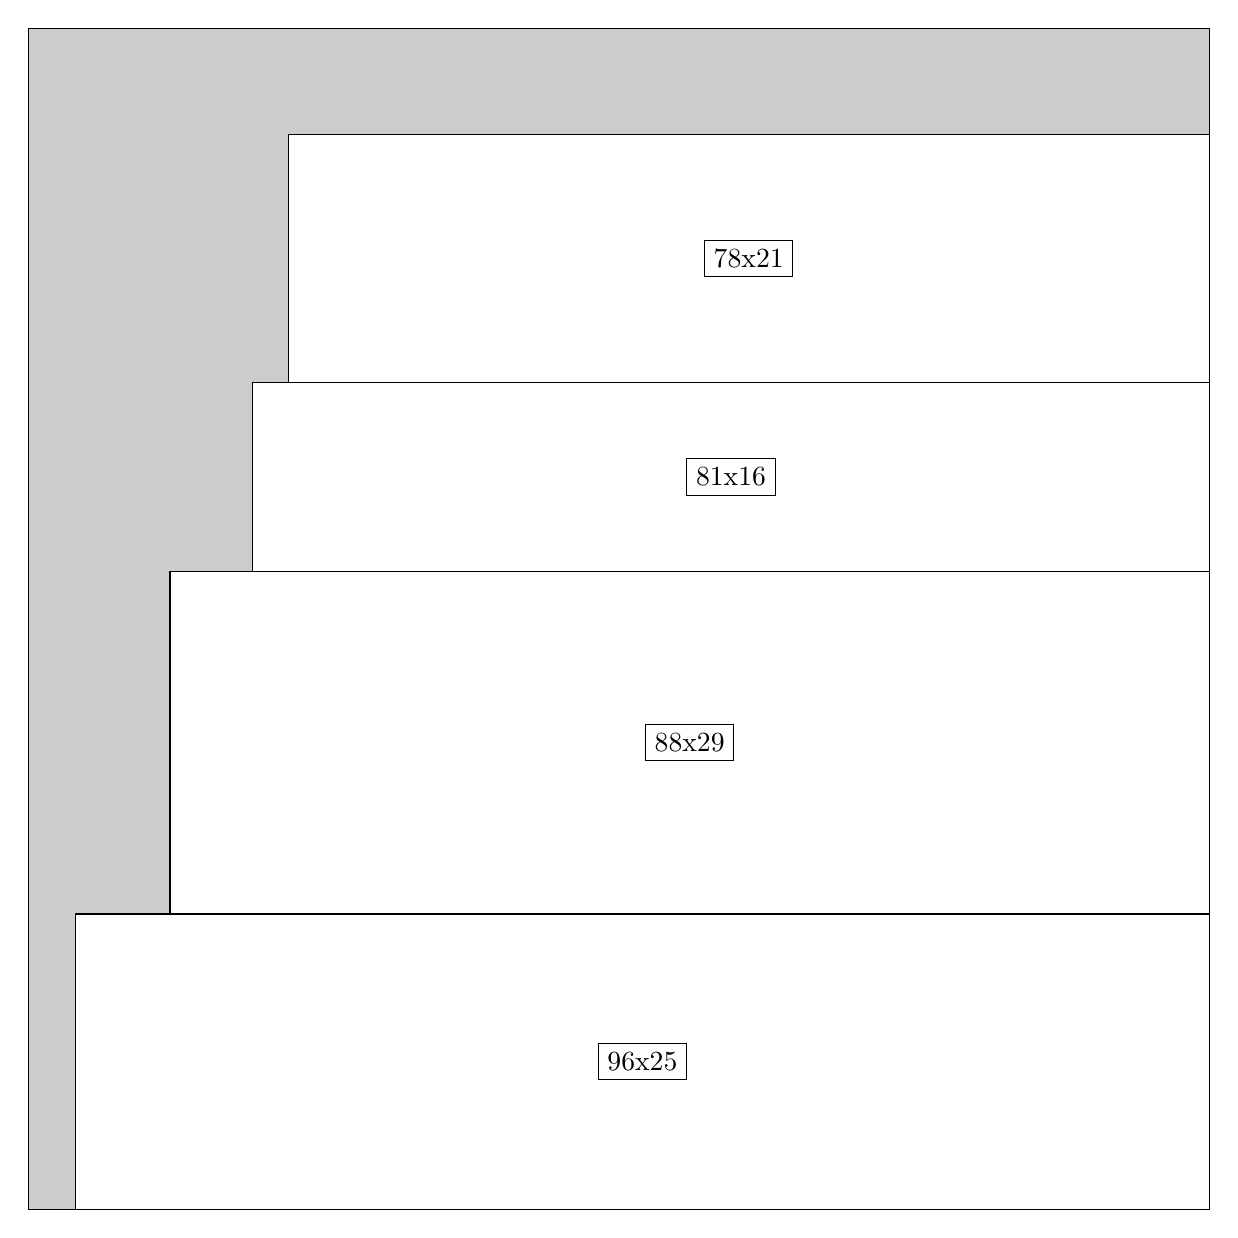
\begin{tikzpicture}[shorten >=1pt,scale=1.0,every node/.style={scale=1.0},->]
\tikzstyle{vertex}=[circle,fill=black!25,minimum size=14pt,inner sep=0pt]
\filldraw[fill=gray!40!white, draw=black] (0,0) rectangle (15.0,15.0);
\foreach \name/\x/\y/\w/\h in {96x25/0.6/0.0/14.399999999999999/3.75,88x29/1.7999999999999998/3.75/13.2/4.35,81x16/2.85/8.1/12.15/2.4,78x21/3.3/10.5/11.7/3.15}
\filldraw[fill=white!40!white, draw=black] (\x,\y) rectangle node[draw] (\name) {\name} ++(\w,\h);
\end{tikzpicture}


w =96 , h =25 , x =4 , y =0 , v =2400
\par
w =88 , h =29 , x =12 , y =25 , v =2552
\par
w =81 , h =16 , x =19 , y =54 , v =1296
\par
w =78 , h =21 , x =22 , y =70 , v =1638
\par
\newpage


\end{document}